\chapter{Identification of Non-photonic Electrons}

We discuss the procedure for identifying electrons in events at STAR and how we remove photonic background. We show the event and track selection criteria and then lastly we will analyze the efficiency for identifying background photonic electrons. The identification of non-photonic electrons (NPE) and efficiency thereof will be critical factors when we construct the NPE-hadron correlations in later chapters.

\section{Outline of the NPE Identification}

This chapter will lay out the general methods for event selection, track selection, electron identification, and the removal of photonic electron background for both Au+Au and p+p collisions.

We start by identifying the dataset and the trigger collections we will use for the analysis. We look at the events and check that the quality of the event is good and that there could be candidate tracks for NPE in the event. We then reconstruct all tracks in the TPC and apply track quality cuts. To identify electrons we rely on the energy loss ($dE/dx$) measured in the TPC and on the hits in the EMC towers and shower max detector. 

The background from photonic electrons will be removed by searching for the opposite signed partner electron. If the primary track is from Dalitz decays or photon conversion in the detector, the partner and primary track should have a low invariant mass. We will also investigate, through simulations, the efficiency for determining the background from photonic electrons.

In the end we will have a sample of electrons which we can use as triggers for measuring NPE-hadron correlations. 

\section{Dataset and Event Selection}

\subsection{Data and Triggers}

In 2011 RHIC collided gold nuclei at $\sqrt{s_{NN}} = 200$ GeV and delivered 9.79 $nb^{-1}$ integrated luminosity similar to what was delivered during the previous year's run (Figure~\ref{fig:Luma}). The STAR detector recorded about 1.1 billion events across all triggers with TPC and BEMC information. In 2012 polarized proton collisions were run in RHIC (the polarization of the beams is not relevant to this analysis) at the same 200 GeV beam energy. RHIC delivered 74.0 $pb^{-1}$ (Figure~\ref{fig:Lumb}) which resulted in 1.7 billion triggered events in STAR. Heavy flavor events are rare and detector efficiencies can be low meaning the NPE analysisis typically constrained by statistics, necessitating large data sets. The Silicon Vertex Tracker (SVT) was removed from STAR resulting in less material near the beam line which cuts down on background from conversions in the detector. This combination of low material and high statisics make runs 11 and 12 (prior to run 14) the best datasets available for the analysis of non-photonic electrons.

\begin{figure}[htbp]
    \begin{subfigure}{0.5\textwidth}
        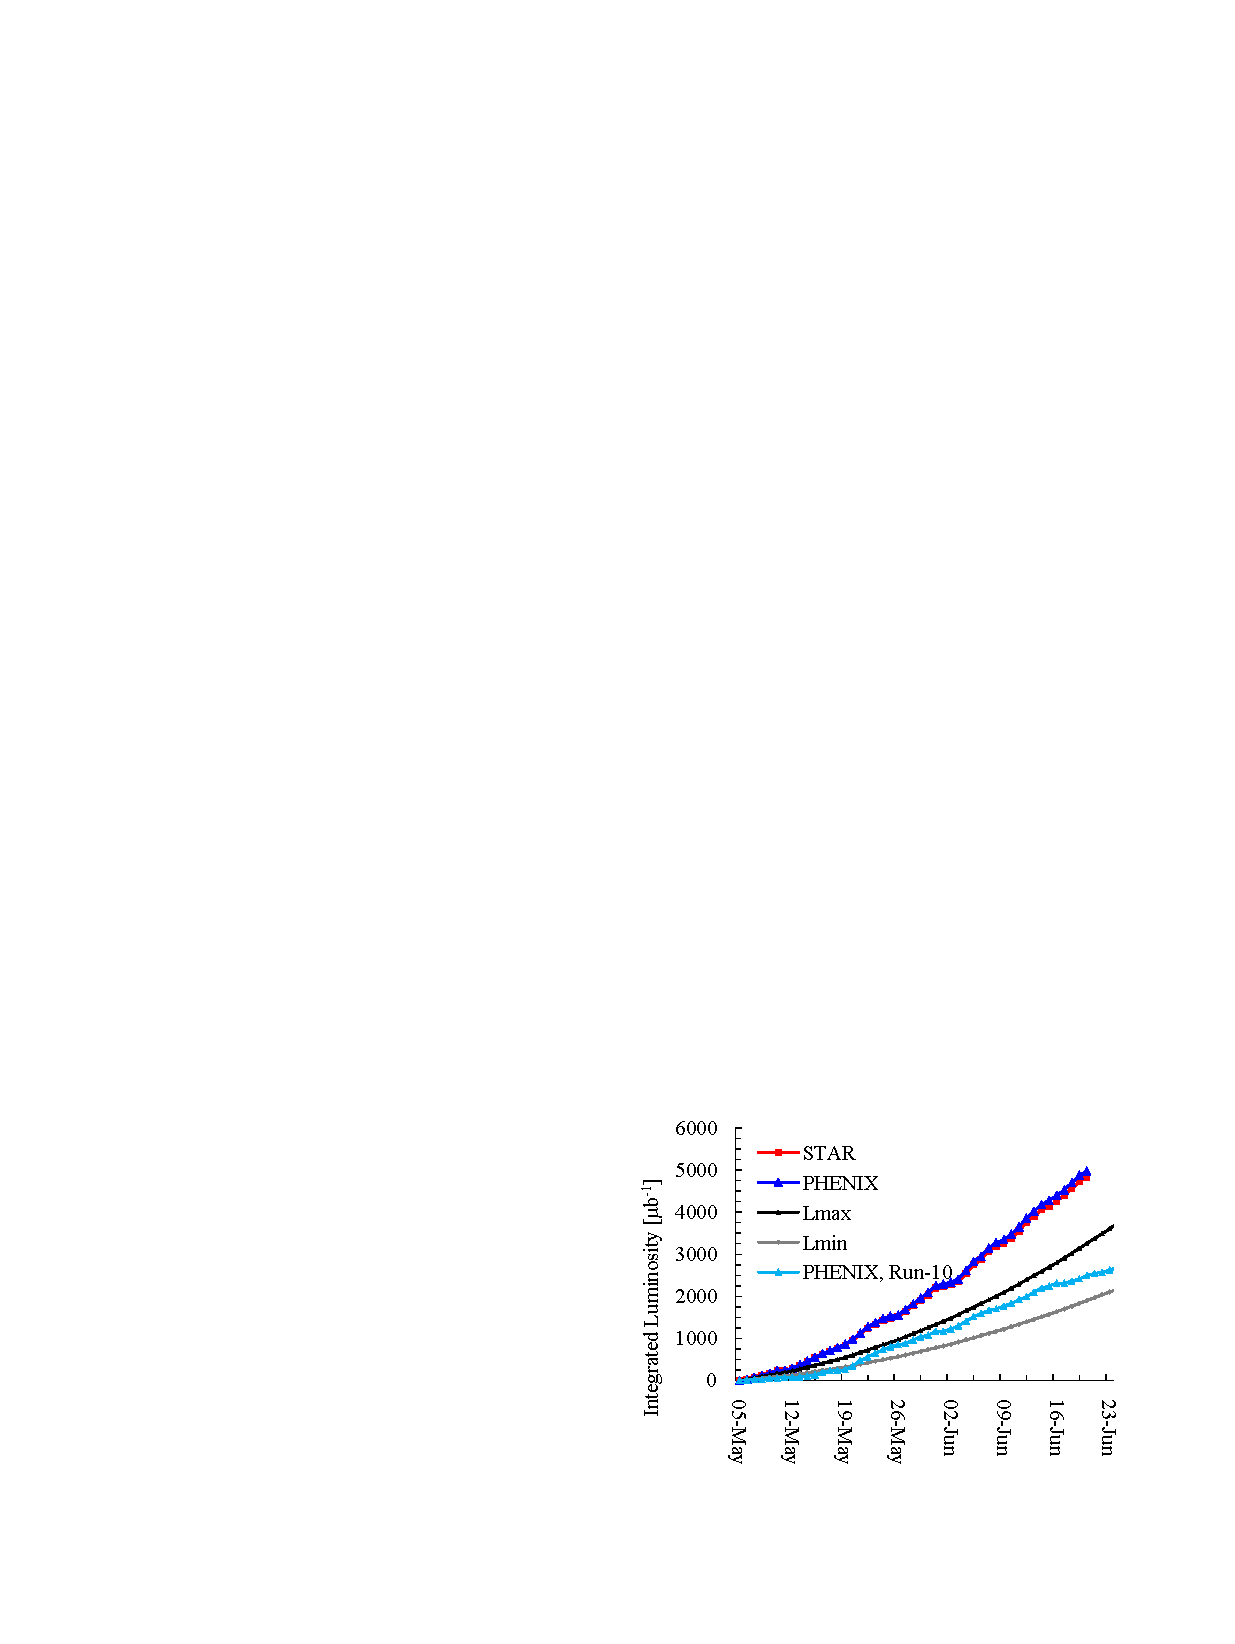
\includegraphics[width=\textwidth]{Plots/NPE/Run11_Lum.pdf}
        \caption{Run 11 Au+Au Integrated Luminosity}
        \label{fig:Luma}
    \end{subfigure}
    \begin{subfigure}{0.5\textwidth}
        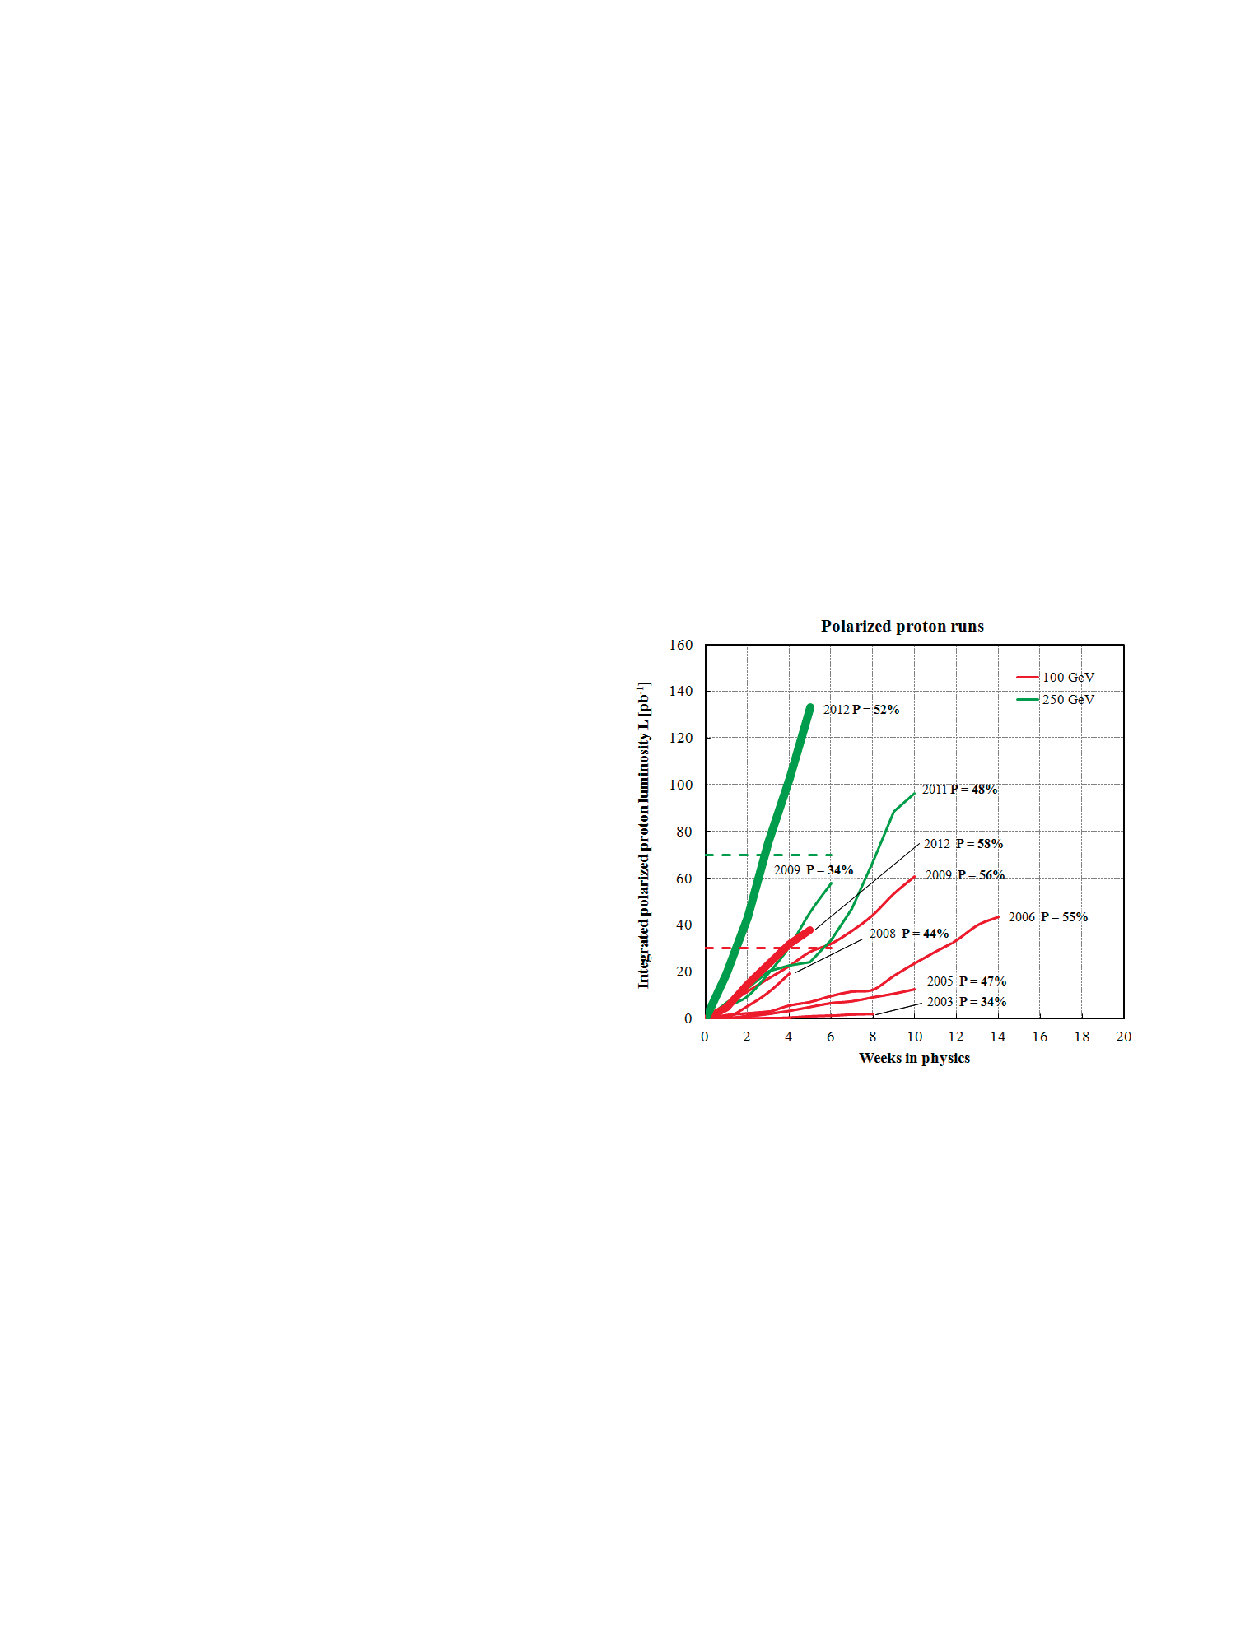
\includegraphics[width=\textwidth]{Plots/NPE/Run12_Lum.pdf}
        \caption{Run 12 p+p Integrated Luminosity}
        \label{fig:Lumb}
    \end{subfigure}
\caption[RHIC Integrated Luminosities in Run11 and Run12]{Integrated luminosities for run 11 and run 12 in RHIC. Left plot shows Au+Au delivered to STAR and PHENIX as well as run 10 in PHENIX for comparison. Right plot shows all p+p runs, run 12 is shown with thick lines.}
\label{fig:RunLum}
\end{figure}

The STAR data acquisition system handles several different triggers the most commonly used is the minimum bias trigger (minbias) which fires based on the coincidence of the STAR vertex position detector(VPD) and Zero Degree Calorimeters (ZDC) these events are prescaled so that only a fixed fraction of triggers are accepted so that the DAQ's data taking rate is not exceeded. STAR can also trigger on hits in the barrel EMC, these are the high tower (HT) triggers. A high tower trigger requires that a hit in a BEMC tower exceeds an ADC threshold determined such that the transverse energy in that tower is high. In run 11 we use the HT triggers NPE11, NPE15, NPE18, and NPE25 which are in increasing order of $E_{T}$. The NPE11 and NPE15 triggers are also prescaled. In p+p we use the BHT0, BHT1, BHT2, and BHT3 triggers, of these only BHT0 is prescaled.

Due to the large dataset sizes it is in our best interest to cut down on the data we need whenever possible. We do this first when we read the data to make BEMC points to match to tracks. Here we look through the tracks in the event and search for electron candidates based on the TPC information only. We throw out events without viable electron candidates. Since these cuts are looser than the electron cuts we will apply later we don't remove events we might actually want and we retain the ability to tighten the cuts later if we need to. After limiting ourselves to high tower triggers and keeping only events with electron candidates we are left with approximately 23 million events in Au+Au and 1.1 million events in p+p.

\subsection{Event Level Cuts}

At the event level we cut on events with vertex too far out of the center of the detector. We use the tracks in the TPC to reconstruct the vertex, we can also measure the vertex with the Vertex Position Detector (VPD). By convention we have the $x$ and $y$ axes as transverse to the beam line. The $z$ axis then runs along the beam. We require that the vertex be no more than 2 cm from the center of the beam pipe in the radial direction, i.e. $\sqrt{(V_x^{TPC})^2 + (V_y^{TPC})^2} \leq$ 2 cm. We also cut on the TPC vertex in the $z$ direction, choosing events with $|V_z^{TPC}| \leq$ 30 cm in Au+Au collisions and $|V_z^{TPC}| \leq$ 40 cm in p+p. Additionally we want to have good agreement between the vertices as measured by the TPC and VPD. We require that the difference between the measured $V_z$ satisfies $|V_z^{TPC} - V_z^{VPD} \leq|$ 4 cm in Au+Au. Figure~\ref{fig:Vertexz} shows the distribution of $V_z^{TPC}$ and the difference in TPC and VPD $V_z$ in Au+Au collisions. In p+p because of lower multiplicity and a wider vertex distribution the measured vertex from VPD is not reliable and thus the cut on the difference of $V_z$ is not used.

\begin{figure}[htbp]
    \begin{subfigure}{0.5\textwidth}
        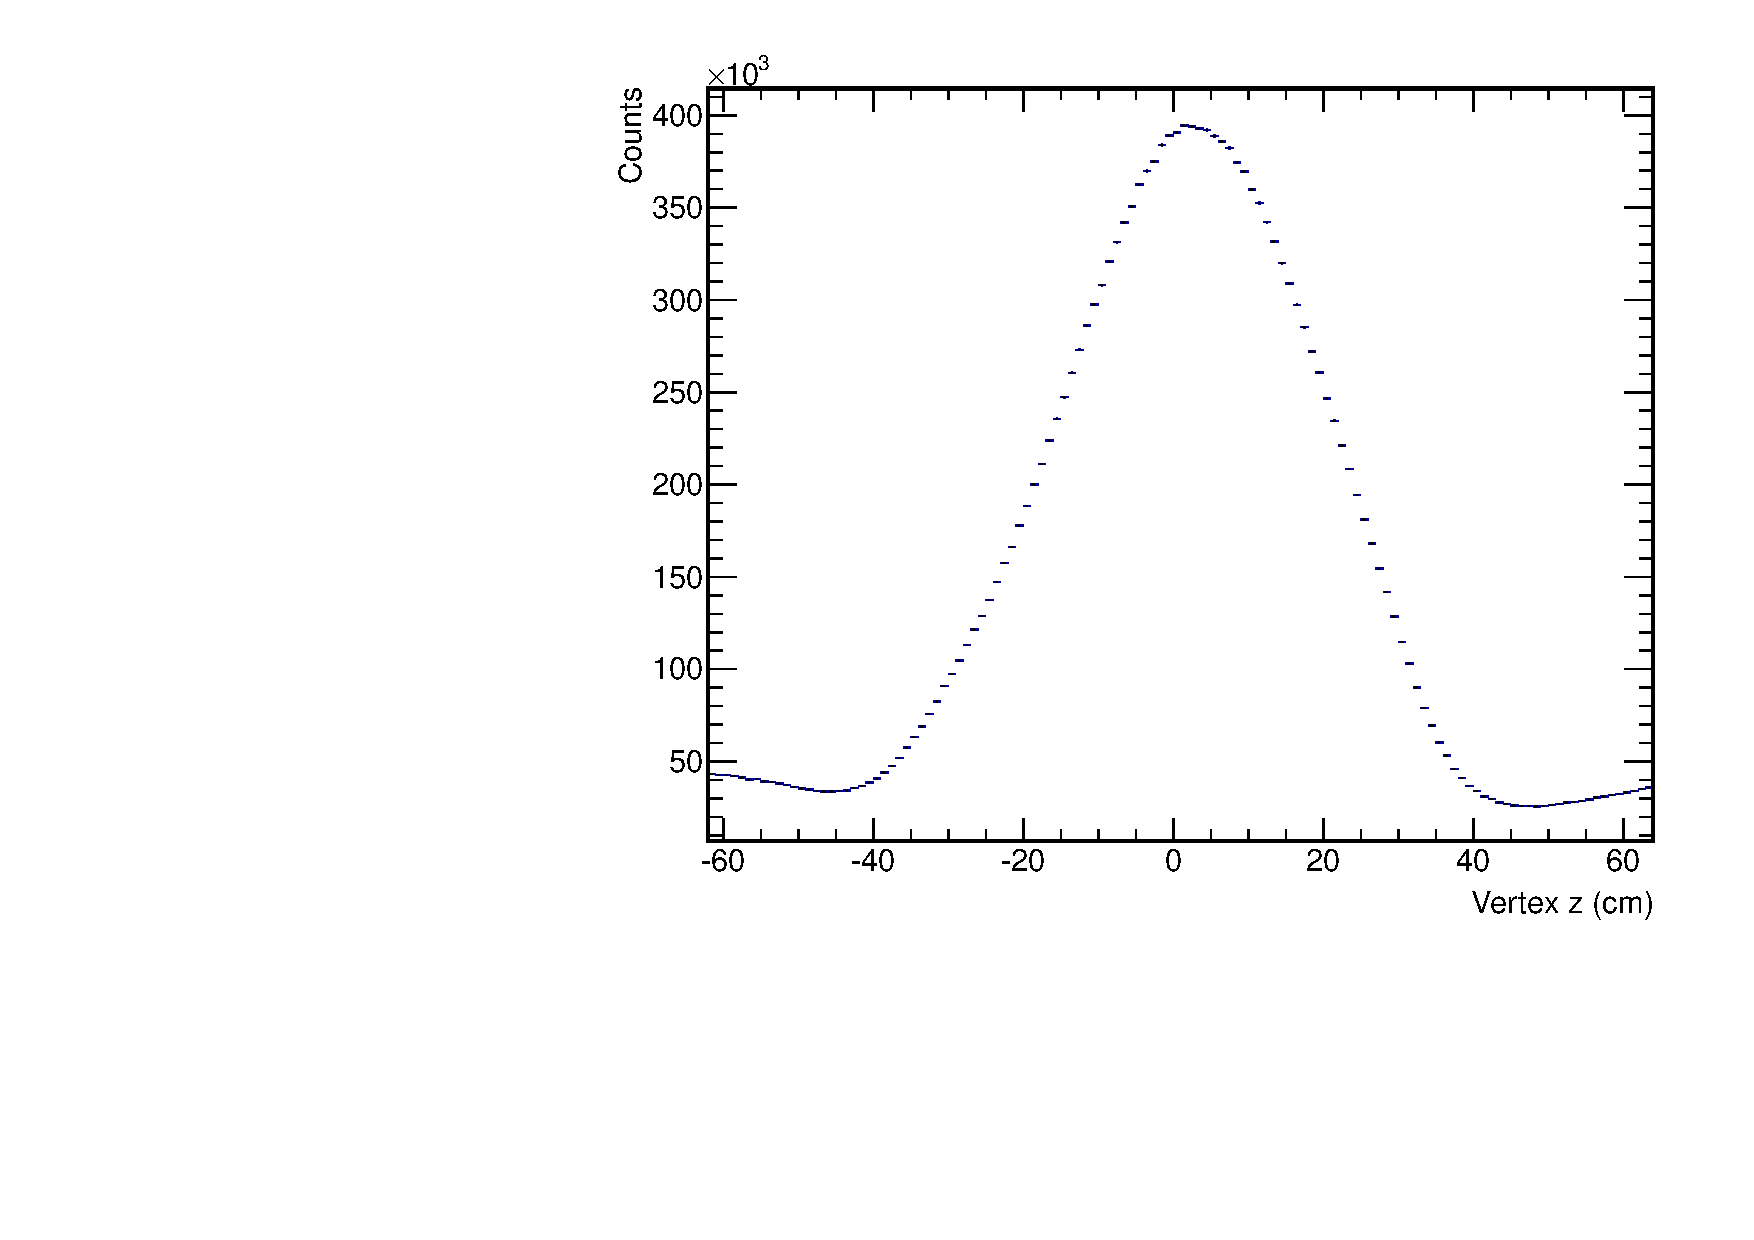
\includegraphics[width=\textwidth]{Plots/NPE/VzAuAu.pdf}
        \caption{$V_{z}^{TPC}$}
        \label{fig:VzAuAu}
    \end{subfigure}
    \begin{subfigure}{0.5\textwidth}
        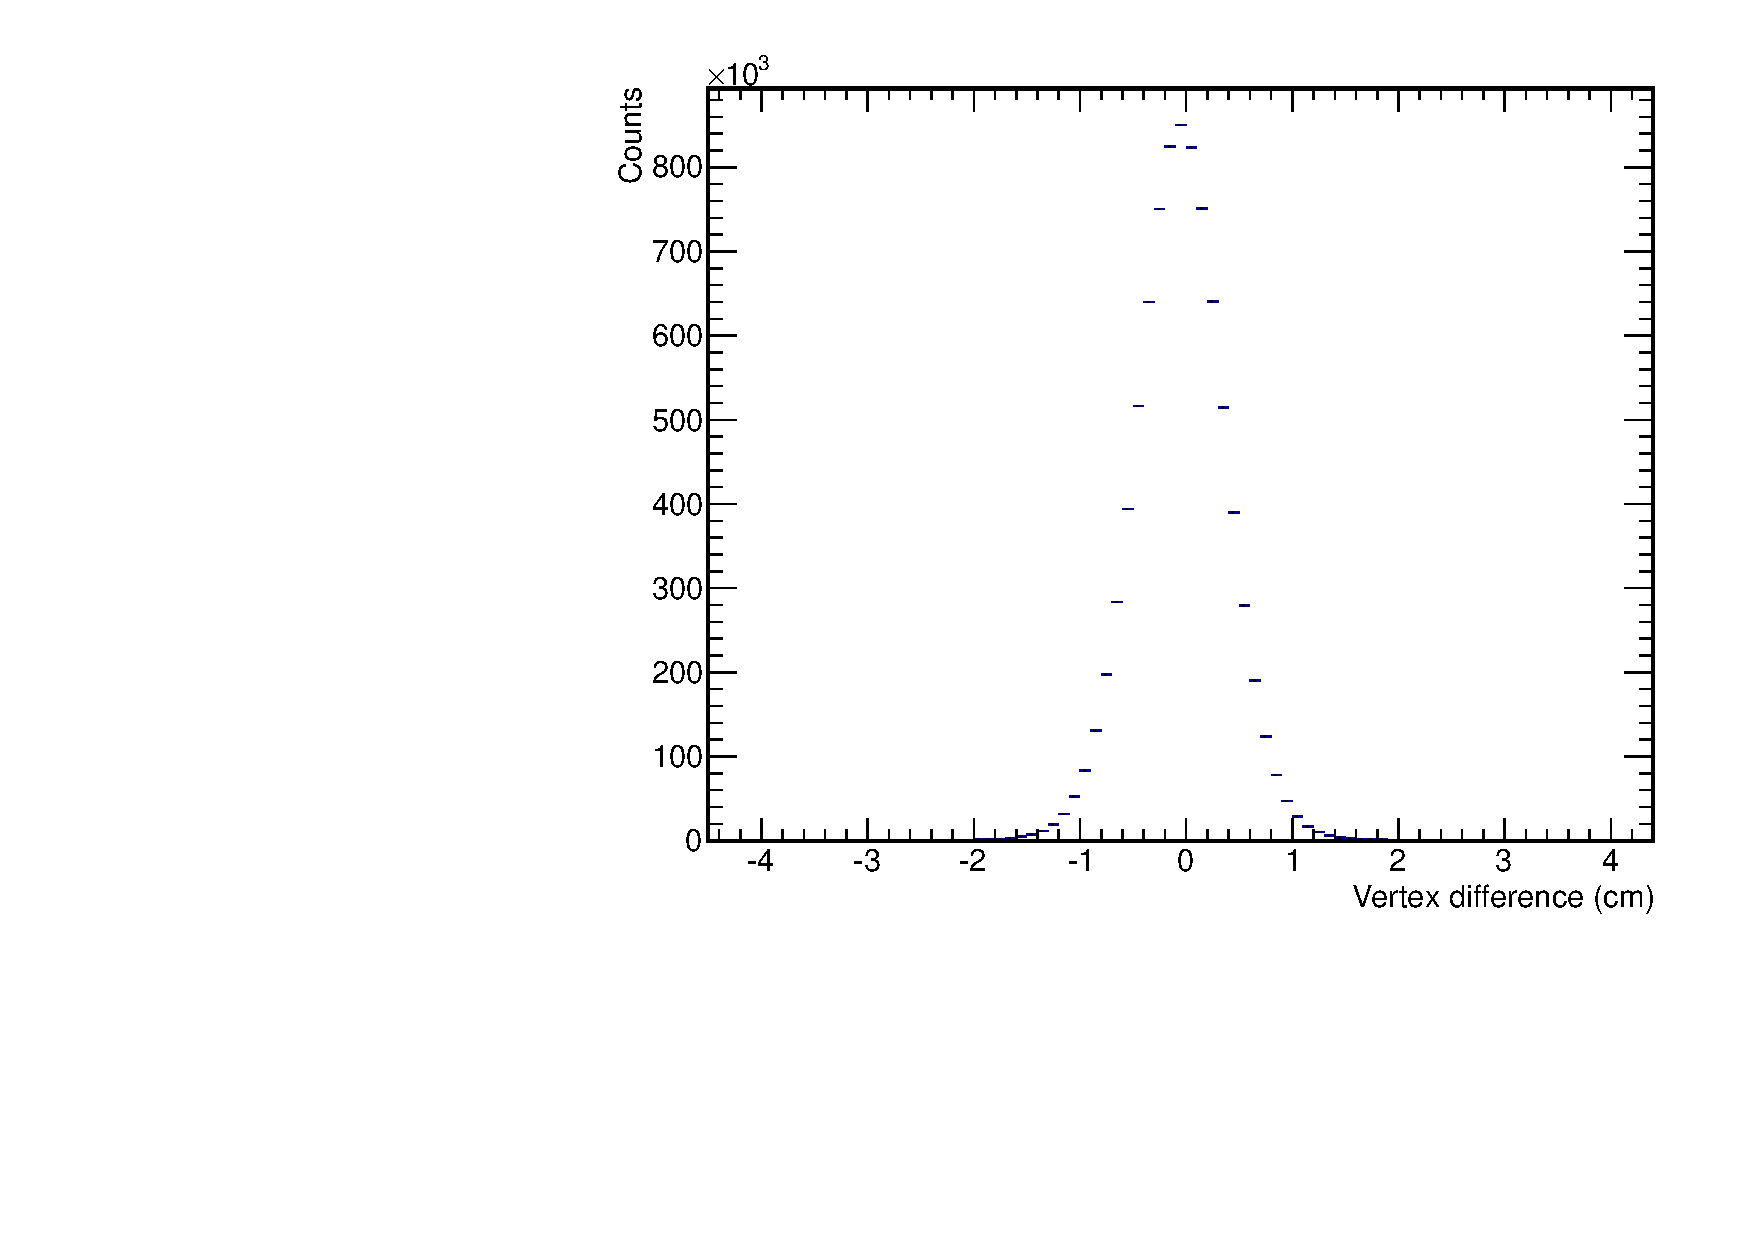
\includegraphics[width=\textwidth]{Plots/NPE/VzDiff.pdf}
        \caption{$V_z^{TPC} - V_z^{VPD}$}
        \label{fig:VertexDiff}
    \end{subfigure}
\caption[TPC $V_z$ and TPC VPD Difference]{Vertex z distribution in run 11 Au+Au. Left plot shows the distribution of the z vertex (cut at $\pm$30 cm), right plot shows the difference between TPC and VPD $V_z$ (cut at $\pm$4 cm).}
\label{fig:Vertexz}
\end{figure}

At the event level we also determine the centrality using the STAR \texttt{StRefMultCorr} which calculates the centrality bin based on the reference multiplicity (refmult), vertex z, run number, and zdc coincidence rate. Figure~\ref{fig:EventCent} shows the event by event distribution of refmult as well as the number of events from each centrality bin used in the NPE analysis.
 
\begin{figure}[htbp]
    \begin{subfigure}{0.5\textwidth}
        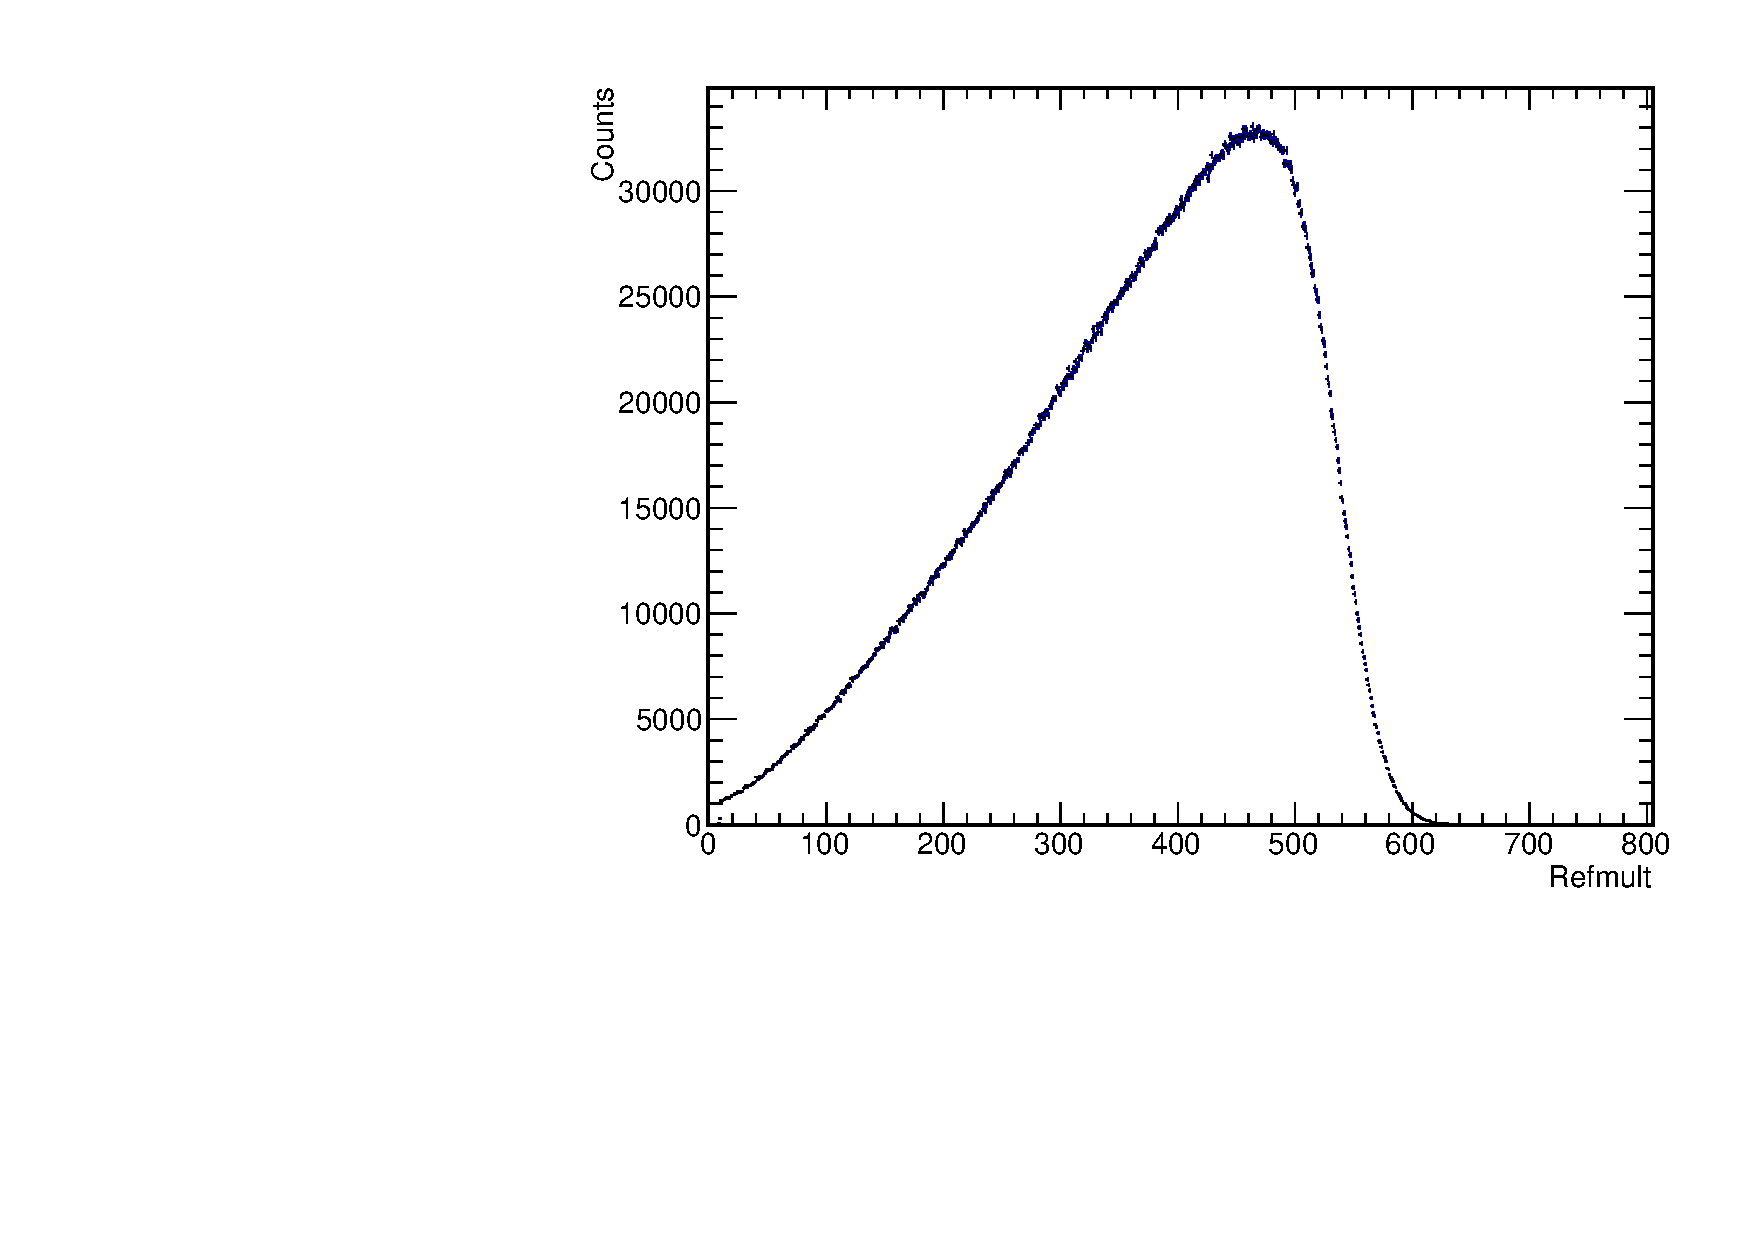
\includegraphics[width=\textwidth]{Plots/NPE/RefmultNPE18.pdf}
        \caption{Reference Multiplicity}
        \label{fig:refmult}
    \end{subfigure}
    \begin{subfigure}{0.5\textwidth}
        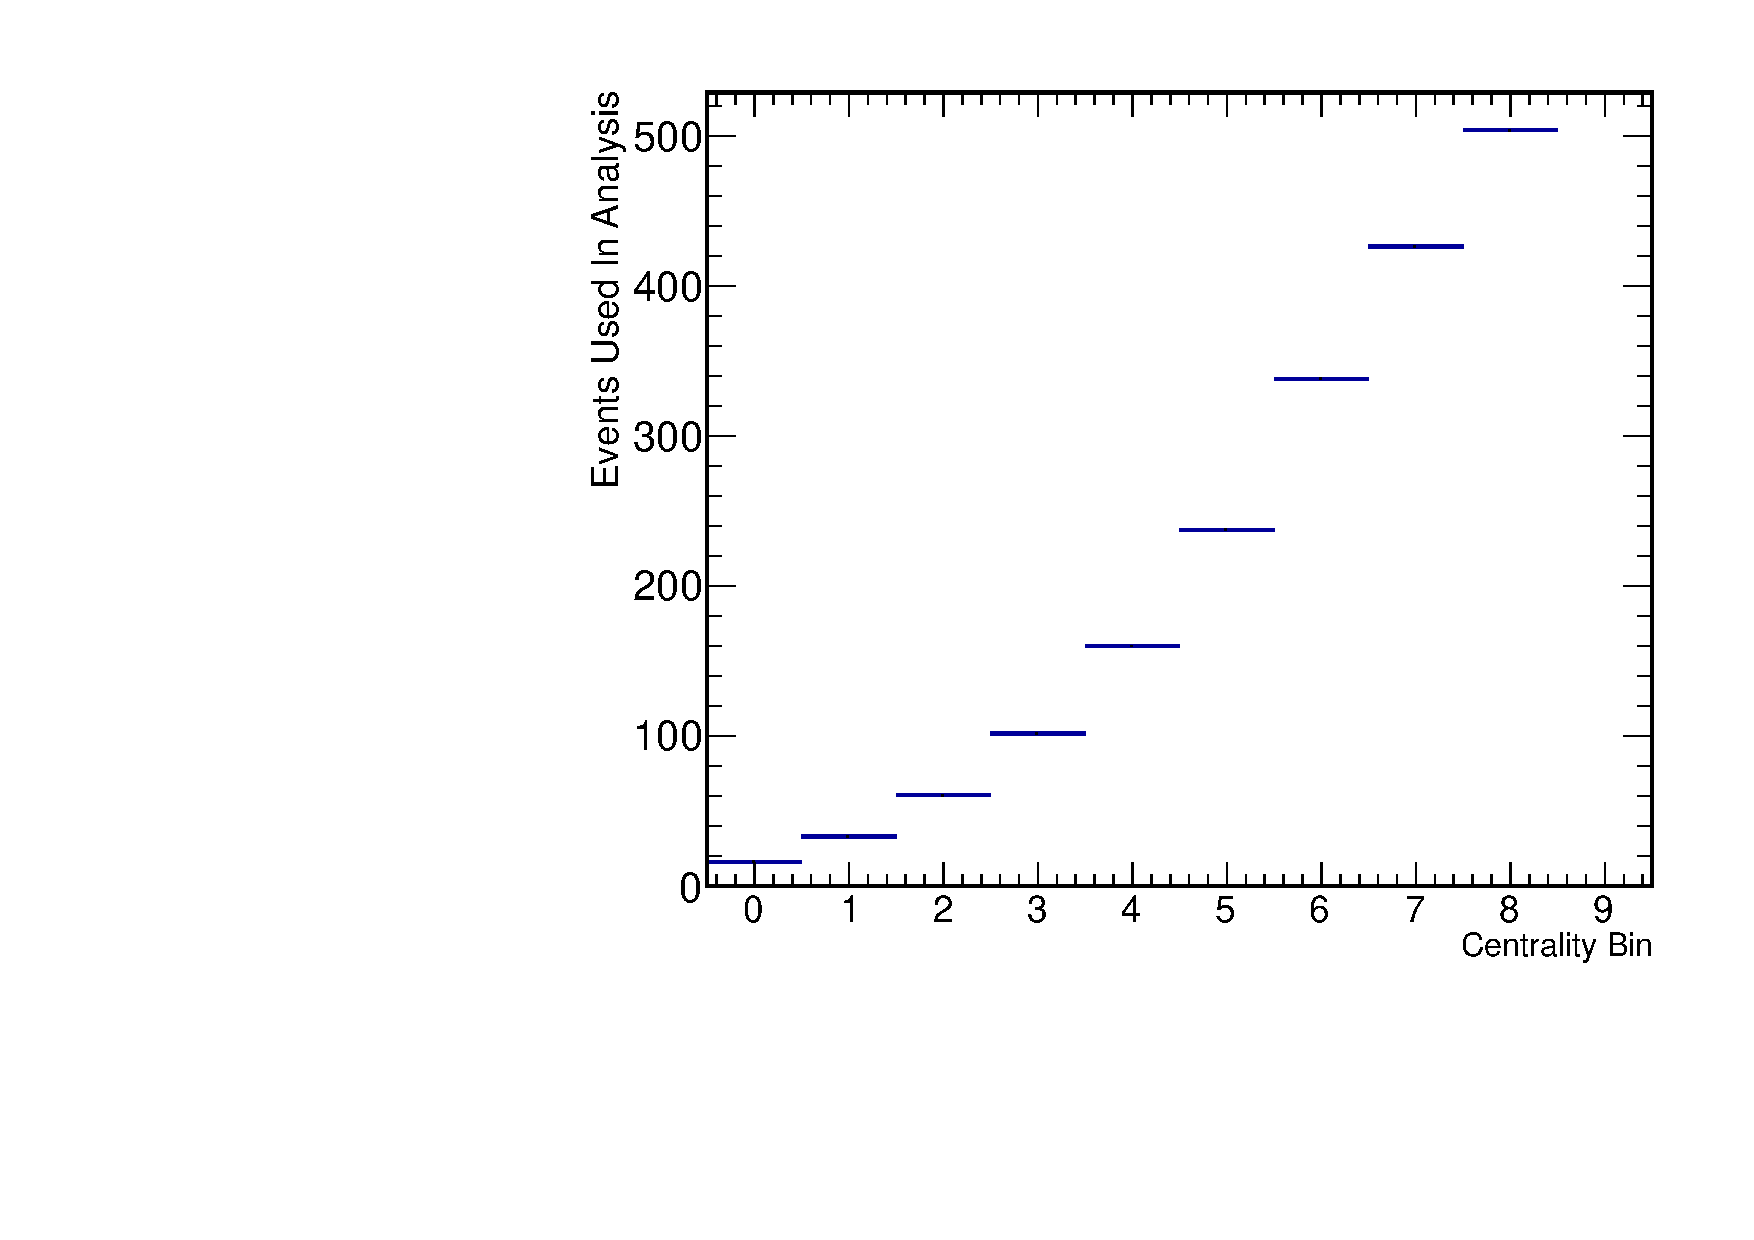
\includegraphics[width=\textwidth]{Plots/NPE/Centrality_dist.pdf}
        \caption{Centrality bins}
        \label{fig:centdist}
    \end{subfigure}
\caption[Refmult and Centrality Distributions]{Reference multiplicity and centrality bin distributions for HT trigger events in Au+Au.}
\label{fig:EventCent}
\end{figure}

\section{Track Reconstruction and TPC Cuts}

\section{BEMC Points and Matching}

\section{Electron Purity}

\section{Photonic Electron Identification}

\section{Photonic Electron Reconstruction Efficiency}
